\chapter{Grundlagen}
In diesem Kapitel werden die für diese Arbeit nötigen Grundlagen hergeleitet und erklärt. Dabei wird besonders auf den verwendeten Radartyp, die entsprechenden Leistungsbetrachtungen und die Phasenregelkreise eingegangen.  
\section{Radar}
Ein Radar versendet eine elektromagnetische Welle und empfängt, falls ein Objekt in Ausbreitungsrichtung vorhanden ist, die davon reflektierte Welle. Aus Unterschieden zwischen beiden Wellen lassen sich verschiedene Informationen, wie Ort und Geschwindigkeit eines Objekts erkennen. Radar\footnote{\textbf{RA}dio \textbf{D}etection \textbf{A}nd \textbf{R}anging} ist dabei die Bezeichnung für diese Form von Erkennungsverfahren und nutzt dabei drei grundlegende physikalische Gesetze von elektromagnetischen Wellen aus:
\begin{description}
\item Definierte Reflexion an Objekten \\
Wenn ein elektrisch leitendes Objekt getroffen wird, kommt es zu einer Reflexion. Diese neue Welle lässt sich mit einem Empfänger erkennen. 
\item Konstante Geschwindigkeit im Freiraum\footnote{Freiraum bezeichnet den mit Luft gefüllten Bereich zwischen Sender und Zielobjekt} \\
Durch konstante Geschwindigkeit lässt sich die über Messung bis zum Erkennen einer reflektierten elektromagnetischen Welle die Entfernung zu einem Objekt bestimmen. 
\item Geradlinige Ausbreitung \\
Durch spezielle Antennen ist es möglich, Winkel zwischen Sender und Objekt zu bestimmen.
\end{description}
Dabei ist der Begriff Radar nur ein Überbegriff für verschiedene Funktionsweisen die die genannten Gesetzmäßigkeiten nutzen. Anschaulich ist das Radarprinzip in Bild dargestellt.

%%BILD FUER HERLEITUNG

Anschaulich ist das Radarprinzip in Bild dargestellt. Dabei muss zwischen einem \textbf{monostatischem} und einem \textbf{bistatischem} Radar unterschieden werden. In einem monostatischem Radar befinden sich Sender und Empfänger am selben Ort. In einem bistatischem Radar ist der Ort unterschiedlich. \\
Um aus Bild einen Zusammenhang zwischen Sende- und Empfangsleistung zu erhalten wird vorrausgesetzt, dass Sender und Empfänger am gleichen Ort sind, es also ein monostatisches Radar ist. Dabei ist die \textbf{Sendeleistung} $P_{S}$ die Leistung der vom Sender erzeugten Welle, die mit dem \textbf{Antennengewinn} $G_{S}$ abgestrahlt wird. Mit \textbf{Entfernung} von Radar zu Objekt $R$ und dem \textbf{Rückstrahlfläche} $\sigma$ wird eine reflektierte Leistung in entgegengesetzter Richtung, also Richtung Radar, vom Objekt abgestrahlt. Die \textbf{reflektierte Leistung} $P_{R}$ ergibt sich demnach zu
\begin{align}
P_{R} = \frac{P_{S} \cdot G_{S} \cdot \sigma}{4\pi \cdot R^2}.
\end{align} Die Empfangsleistung ergibt sich über die reflektierte Leistung und die \textbf{Antennenwirkfläche} $A$ wobei für $A{W}$ gilt mit dem \textbf{Antennengewinn} der Empfangsantenne $G_{e}$\footnote{In diesem Fall ist die Empfangsantenne und die Sendeantenne identisch, allerdings lässt sich die Herleitung verallgemeinern, wofür diese Unterscheidung notwendig ist}. 
\begin{align}
A = \frac{\lambda^2 \cdot G_{e}}{4\pi}.
\end{align}
Dadurch ergibt sich die über die \textbf{Empfangsleistungsdichte} $S_{E}$, wobei 
\begin{align}
S_{E} = \frac{P_{R}}{4\pi \cdot R^2}.
\end{align}
ist, die 
\textbf{Empfangsleistung} $P_{E}$ mit
\begin{align}
P_{E} = S_{E}\cdot A_{W}.
\end{align}
und mit obigen Gleichungen
\begin{align}
P_{E} = \frac{P_{S} \cdot G_{S} \cdot G_{E} \cdot \sigma \cdot \lambda^2}{(4\pi)^3\cdot R^4}
\end{align}
die \textbf{Radargleichung}\footnote{Einzige Einschränkung ist hier, dass Sender und Empfänger die gleiche Entfernung vom Ziel haben müssen. Mit obigen Einschränkungen ist zusätzlich $G_{S} = G_{E}$ wodurch sich die Radargleichung weiter vereinfacht.}.
Durch Umstellung nach $R$ unter Berücksichtigung der \textbf{minimal Empfangsleistung} $P_{E,min}$\footnote{$P_{E,min}$ ist dabei proportional zur \textbf{Empfängerbandbreite}
$B$, der \textbf{Empfängerrauschzahl} $F$ und dem \textbf{minimalen Signal-zu-Rausch-Verhältnis} $SNR_{min}$.} ergibt sich eine \textbf{maximale Radarreichweite} $R_{max}$ mit
\begin{align}
R_{max} = \sqrt[4]{\frac{P_{S} \cdot G_{E}\cdot G_{S} \cdot \lambda^2 \cdot \sigma}{P_{E,min} \cdot (4\pi)^3}}.
\end{align}
Das Verhältnis von ausgesendeter Leistung und empfangener Leistung bezeichnet die \textbf{Freiraumdämpfung} $F$ oder FSPL\footnote{\textbf{F}ree\textbf{S}pace\textbf{P}ath\textbf{L}oss}. Dabei ist
\begin{align}
F = \frac{P_{E}}{P_{S}} = \left(\frac{4\pi \cdot R}{\lambda}\right)^2.
\end{align} 
und mit \textbf{Lichtgeschwindigkeit} c sowie \textbf{Frequenz} f
\begin{align}
c = \lambda \cdot f.
\label{eq:fzulambda}
\end{align}
die Freiraumdämpfung
\begin{align}
F(f,r) = \left(\frac{4\pi \cdot R \cdot f}{c}\right)^2
\end{align}
eine Funktion in Abhängigkeit der Frequenz, und dem Abstand $R$. Diese Frequenz bleibt konstant. Häufig wird $F(f)$ in dB und mit der englischen Bezeichnung bezeichnet, demnach ist
\begin{align}
\text{FPSL(dB)} &= 10\log_{10}\left(\frac{4\pi \cdot R \cdot f}{c}\right)^2 \notag \\
&= 20 \log_{10}\left( R \right) + 20 \log_{10}\left( f \right) - 147,55 .
\end{align}

\section{Radartypen}
Radarsysteme lassen sich in Impuls- und Dauerstrichradarsysteme unterteilen. Das Impulsradar ist hier nicht beschrieben, da es für die weitere Arbeit keine  Verwendung hat. Als Vertreter der Dauerstrichradare wird besonders auf das FMCW Radar eingegangen.

\subsection{Zielentfernung}
Das Radar sendet eine Signal in den Freiraum aus und misst die Zeit, bis das reflektierte Signal detektiert wird. Dieser \textbf{Zeitunterschied} $\Delta t$ gibt mit Hilfe der konstanten \textbf{Lichtgeschwindigkeit} $c$ den \textbf{Abstand} $R$ von Radar zu Objekt über
\begin{align}
R = \frac{c \cdot \Delta t}{2} 
\end{align} 
an. Bezieht man zusätzlich eine konstante Radialgeschwindigkeit des Ziels mit ein, gilt für den Abstand 
\begin{equation}
R(t) = R_{0} - v_{r} \cdot \left( t-t_{0}\right).
\end{equation}
Für den Laufzeitunterschied gilt demnach nach \cite[Gl. 3.1.11]{HuderRadar}
\begin{equation}
\Delta t = \frac{2R}{c_{0}}
		 = \frac{2}{c_{0}}\left(R_{0} - v_{r} \cdot \left( t-t_{0}\right)\right)
\label{eq:AbstandZuDeltaT}
\end{equation}

\subsection{Dauerstrichradar}
Das Dauerstrichradar, auch CW-Radar\footnote{\textbf{C}ontinuous  \textbf{W}ave Radar} sendet im Gegensatz zum Puls-Radar ein kontinuierliches Signal aus. Durch Laufzeitunterschiede des empfangenen und gesendeten Signals lässt sich so der Abstand zu einem Ziel bestimmen. In Abbildung\ref{fig:cwradar} ist das CW-Radar als Blockschaltbild dargestellt.
\begin{figure}[tbp]
  \centering
  \tikzset{%
	% Self defined bulding blocks. 
	% Nevertheless circutikz has implemented filters, couplers and other components since version 0.4, they are mostly implemented as bipoles.
	% The usage of bipoles: \draw (start) to[lowpass/amp/adc,....] (end).
	% The problem is, that if one wants to use arrows, the arrows in bipoles can not be sat manual (fixed in circuitikz source) AND THEY ARE NOT CONSISTENT
	% Also it's quite a mess, which component is a monopole, simple block, bipol, quad/triple etc
	% Following are a few examples on how to define your own blocks. 
	%
	% % % % % % % % % % % % % % % % % % % % % % % % % % % % % % % % % % % % % % % % % % % % % % % % % % % % % % % % % % % % % % % % % % % % %
	% % % % % % % % % % % % % % % % % % % % % % % % % % % % % % % % % % % % % % % % % % % % % % % % % % % % % % % % % % % % % % % % % % % % %
	% % % % % % % % % % % % % % % % % % % % % % % % % % % % % % % % % % % % % % % % % % % % % % % % % % % % % % % % % % % % % % % % % % % % %
	% % % % % % % % % % % % % % % % % % % % % % % % % % % % % % % % % % % % % % % % % % % % % % % % % % % % % % % % % % % % % % % % % % % % %
	%
	% Standard block definition, the width and height is adopted from the circutizk source code, so don't mind the strange values. Also the linewidth is set according to the circutrikz source code.
	block/.style    	= 	{draw, fill=white, thick, rectangle, minimum height = 0.98cm, minimum width = 0.98cm, node distance=2.5cm, line width=1.5pt},
	%
	% Standard circular block
	circleblock/.style	= 	{draw, fill=white, thick, circle, minimum width = 0.98cm,  line width=1.5pt, node distance=2.5cm},
	%
	% Label for circuitikz nodes, as they're reference is in the middle and not on the outer edge of the node....
	circuitikzlabel/.style	=	{label={[label, label distance=0.5cm]#1}},
	%
	%
	%
	% VCO/Oscillator 
	myVCO/.style			= 	{circleblock, path picture={%
		\draw[line width=0.75pt] 	($(path picture bounding box.west)+(0.09cm,0)$) sin ($(path picture bounding box.center)-(0.2cm,-0.2cm)$) cos  (path picture bounding box.center) sin ($(path picture bounding box.center)-(-0.2cm,0.2cm)$) cos ($(path picture bounding box.east)-(0.09cm,0)$);
		}
	},
	% Amplifier, as circuitikz does only provite amplifiers as 2-ports/bipoles
	myAMP/.style		= 	{block, node distance=2.5cm, path picture={%
		\draw[fill=white, line width=0.75pt] ($(path picture bounding box.center)+(0.7em,0)$) -- ($(path picture bounding box.center)-(0.7em,-0.7em)$) -- ($(path picture bounding box.center)-(0.7em,0.7em)$)  -- cycle;
		}
	},
	% Block	
	myBlock/.style    	= 	{draw, fill=white, thick, rectangle, minimum height = 0.98cm, minimum width = 0.98cm, node distance=2.5cm, line width=1.5pt},
	myBigBlock/.style    	= 	{draw, fill=white, thick, rectangle, minimum height = 0.98cm, minimum width = 2.94cm, node distance=2.5cm, line width=1.5pt},	
	% Same for ADC
	myADC/.style 	=	{block, path picture={%
		\draw[line width=0.75pt] 	(path picture bounding box.south west) -- (path picture bounding box.north east);
		\node[] at ($(path picture bounding box.center)+(-.5em,.5em)$) () {D};
		\node[] at ($(path picture bounding box.center)+(.5em,-.5em)$) () {A};
		} 
	},
	% Same for filters
	myLP/.style	=	{block, path picture={%
		%Sine-Waves
		\draw[line width=.75pt] 	($(path picture bounding box.west)+(0.3em,0)$) sin ($(path picture bounding box.center)-(0.50em,-0.3em)$) cos  (path picture bounding box.center) sin ($(path picture bounding box.center)-(-0.50em,0.3em)$) cos ($(path picture bounding box.east)-(0.3em,0)$);
		\draw[line width=0.75pt] 	($(path picture bounding box.west)+(0.3em,-0.65em)$) sin ($(path picture bounding box.center)-(0.50em,0.35em)$) cos  ( $(path picture bounding box.center)-(0,0.65em)$) sin ($(path picture bounding box.center)-(-0.50em,0.95em)$) cos ($(path picture bounding box.east)-(0.3em,0.65em)$);
		\draw[line width=0.75pt] 	($(path picture bounding box.west)+(0.3em,0.65em)$) sin ($(path picture bounding box.center)-(0.50em,-0.95em)$) cos  ( $(path picture bounding box.center)+(0,0.65em)$) sin ($(path picture bounding box.center)-(-0.50em,-0.35em)$) cos ($(path picture bounding box.east)-(0.3em,-0.65em)$);
		% Cancelation
		\draw[line width=0.75pt] 	($(path picture bounding box.center)-(0.2em,0.2em)$) -- (path picture bounding box.center) -- ($(path picture bounding box.center)+(0.2em,0.2em)$) ;
		\draw[line width=0.75pt] 	($(path picture bounding box.center)-(0.2em,-0.45em)$) -- ($(path picture bounding box.center)+(0,0.65em)$) -- ($(path picture bounding box.center)+(0.2em,0.85em)$) ;
		}
	},
}
\begin{tikzpicture}[line width=0.7pt,>=latex,node distance=2.5cm]
	% First: All building blocks are placed relative to the first component
	\draw (0,0)
		node[myVCO, label={above:Signalgenerator}] (oszi) {}
		% As the coupler ports are not in the middle, based on the size (again extraceted from circutikz source code), an yshift is perfomed to have the input on the same height as the output of the oszillator. The xshift is used to place the VCO and ADC on the same y-value after all.
		% Undo the yshift as the output of the coupler is on the same height as the input of the amplifier
		node[myBlock, right of=oszi,  node distance=5cm, label={above:Sender}] (pa) {$P_{S}$}
		% Circulator is rotated that the ports are on the correct position, normally ports are arranged as follows:
		% 
		%				  o------------o
		%						|
		%						o
		node[circulator, below right of=pa, xshift = 3cm, rotate=90,] (circ) {}
		node[antenna, right of = circ] (antenna) {}
		node[myBlock, below left of=circ,  label={below:Empfänger}] (lna) {$P_{E}$}
		% Used redefinition of label, otherwise the label would be overlapping with the mixer shape
		node[mixer, below of=pa,yshift = -1cm  , circuitikzlabel={below:Mischer}] (mixer) {}
		node[myLP, left of=mixer, label={below:Tiefpass}] (lowpass) {}
		node[myADC, left of = lowpass,node distance=2.5cm, label ={below:Signalverarbeitung}](Sig){}		
		;
		
	% Connect everything together
	\draw[->] (oszi) -- node[above]{$u_{S}(t)$}(pa.west);

	%\draw[] (coupler.1) -| ++(-0.5cm,-0.1cm) node[match, rotate=-90, yscale=-1] {};
	\draw[->] (pa.east) -| node[above left]{$u_{S}(t)$}(circ.2);
	\draw[-] (circ.3) -- (antenna);
	\draw[->] (circ.1) |- node[above left]{$u_{E}(t)$}(lna.east);
	\draw[->] (lna.west) -- node[above]{$u_{E}(t)$}(mixer.east);
	\draw[->] (mixer.west)  -- node[above]{$u_{M}(t)$} (lowpass.east);
	\draw[->] (lowpass.west) -- node[above]{$u_{TP}(t)$}(Sig.east);
	\draw[->] (pa.south) -- node[right]{$u_{S}(t)$}(mixer.north);

\end{tikzpicture}

  \caption{CW-Radar Blockdiagramm}
  \label{fig:cwradar}
\end{figure}
Das Sendesignal $u_{S}(t)$ wird versendet. Das empfangene Signal $u_{E}(t)$ gelangt in den Mischer. Im Mischer wird das empfangene Signal mit dem ursprünglichen Signal gemischt. Daraus ergibt sich das Mischsignal $u_{M}(t)$. Das Mischsignal wird in dem nachfolgenden Tiefpass gefiltert. Das daraus entstehende Tiefpasssignal $u_{TP}(t)$ wird weiterverarbeitet und digitalisiert. \\
Ist das Sendesignal $u_{S}(t)$ mit
\begin{align}
u_{S}(t) =  u_{S} \cos\left( \omega_{S}t + \varphi_{S}\right)
\end{align} 
cosinus-förmig mit Phase $\varphi_{S}$ und Winkelgeschwindigkeit $\omega_{S}$ mit 
\begin{align}
\omega_{S} = 2 \pi f_{s}
\end{align}
und das Empfangssignal  $u_{E}(t)$ 
\begin{align}
u_{E}(t) =  u_{E} \cos\left( \omega_{S}\left(t-\Delta t\right) + \varphi_{S}+\varphi_{E}\right) 
\end{align}
ergibt sich im Mischer ein Mischsignal $u_{M}(t)$ mit
\begin{align}
u_{M}(t) = u_{S}(t)\cdot u_{E}(t) = u_{S} u_{E} \cos\left( \omega_{S}t + \varphi_{S}\right)\cdot \cos\left( \omega_{S}\left(t-\Delta t\right) + \varphi_{S}+\varphi_{E}\right).
\end{align}
Wird die trigonometrische Beziehung 
\begin{align}
\cos \alpha \cdot \cos \beta = \frac{1}{2} \left( \cos \left( \alpha + \beta \right) + \cos \left( \alpha - \beta \right) \right)
\end{align}
betrachtet, ergibt sich für das Mischsignal zwei Frequenzen. Zum Einen die Summe der Frequenzen $2\omega_{s}$ zum Anderen die Subtraktion $-\omega_{s}$. Der Tiefpass wird darauf ausgelegt, dass 
\begin{align}
f_{g,TP} = 2f_{s}
\end{align}
gilt.
Es ist nach \cite[S.43,S.44]{HuderRadar} das Tiefpass-Ausgangssignal $u_{TP}(t)$
\begin{align}
u_{TP}(t) = u_{TP} \cos \left( -\omega_{s} \Delta t + \varphi_{Z}\right)
\end{align} und mit Gleichung \ref{eq:AbstandZuDeltaT} ist
\begin{align}
u_{TP}(t) = u _{TP} \cdot \cos \left( \frac{2 \omega_{S} }{c_{0}}\cdot \left( -R_{0} + v_{r}\cdot t - 2 v_{r}\cdot t_{0}\right) +\varphi_{E}\right). 
\end{align}
Ist die Radialgeschwindigkeit $v_{r}$ gleich Null, also keine Bewegung der Sender/Empfängersysteme oder des Ziels, ergibt sich ein konstantes Ausgangssignal am Tiefpass. Dieses konstante Signal lässt sich in die Entfernung zum Ziel umrechnen. 
\subsection{Dauerstrichradar mit Frequenzmodulation}
Das Dauerstrichradar mit Frequenzmodulation, auch FMCW\footnote{\textbf{F}requency \textbf{M}odulated \textbf{C}ontinous \textbf{W}ave}-Radar genannt, beschreibt ein Dauerstrichradar, in welchem das Sendesignal frequenzmoduliert und nicht amplitudenmoduliert wird. Dabei ist der gerätetechnische Aufbau in Abbildung \ref{fig:FMCWRadar} dargestellt. 
\begin{figure}[tbp]
  \centering
  \tikzset{%
	% Self defined bulding blocks. 
	% Nevertheless circutikz has implemented filters, couplers and other components since version 0.4, they are mostly implemented as bipoles.
	% The usage of bipoles: \draw (start) to[lowpass/amp/adc,....] (end).
	% The problem is, that if one wants to use arrows, the arrows in bipoles can not be sat manual (fixed in circuitikz source) AND THEY ARE NOT CONSISTENT
	% Also it's quite a mess, which component is a monopole, simple block, bipol, quad/triple etc
	% Following are a few examples on how to define your own blocks. 
	%
	% % % % % % % % % % % % % % % % % % % % % % % % % % % % % % % % % % % % % % % % % % % % % % % % % % % % % % % % % % % % % % % % % % % % %
	% % % % % % % % % % % % % % % % % % % % % % % % % % % % % % % % % % % % % % % % % % % % % % % % % % % % % % % % % % % % % % % % % % % % %
	% % % % % % % % % % % % % % % % % % % % % % % % % % % % % % % % % % % % % % % % % % % % % % % % % % % % % % % % % % % % % % % % % % % % %
	% % % % % % % % % % % % % % % % % % % % % % % % % % % % % % % % % % % % % % % % % % % % % % % % % % % % % % % % % % % % % % % % % % % % %
	%
	% Standard block definition, the width and height is adopted from the circutizk source code, so don't mind the strange values. Also the linewidth is set according to the circutrikz source code.
	block/.style    	= 	{draw, fill=white, thick, rectangle, minimum height = 0.98cm, minimum width = 0.98cm, node distance=2.5cm, line width=1.5pt},
	%
	% Standard circular block
	circleblock/.style	= 	{draw, fill=white, thick, circle, minimum width = 0.98cm,  line width=1.5pt, node distance=2.5cm},
	%
	% Label for circuitikz nodes, as they're reference is in the middle and not on the outer edge of the node....
	circuitikzlabel/.style	=	{label={[label, label distance=0.5cm]#1}},
	%
	%
	%
	% VCO/Oscillator 
	myVCO/.style			= 	{circleblock, path picture={%
		\draw[line width=0.75pt] 	($(path picture bounding box.west)+(0.09cm,0)$) sin ($(path picture bounding box.center)-(0.2cm,-0.2cm)$) cos  (path picture bounding box.center) sin ($(path picture bounding box.center)-(-0.2cm,0.2cm)$) cos ($(path picture bounding box.east)-(0.09cm,0)$);
		}
	},
	% Amplifier, as circuitikz does only provite amplifiers as 2-ports/bipoles
	myAMP/.style		= 	{block, node distance=2.5cm, path picture={%
		\draw[fill=white, line width=0.75pt] ($(path picture bounding box.center)+(0.7em,0)$) -- ($(path picture bounding box.center)-(0.7em,-0.7em)$) -- ($(path picture bounding box.center)-(0.7em,0.7em)$)  -- cycle;
		}
	},
	% Block	
	myBlock/.style    	= 	{draw, fill=white, thick, rectangle, minimum height = 0.98cm, minimum width = 0.98cm, node distance=2.5cm, line width=1.5pt},
	myBigBlock/.style    	= 	{draw, fill=white, thick, rectangle, minimum height = 0.98cm, minimum width = 2.94cm, node distance=2.5cm, line width=1.5pt},	
	% Same for ADC
	myADC/.style 	=	{block, path picture={%
		\draw[line width=0.75pt] 	(path picture bounding box.south west) -- (path picture bounding box.north east);
		\node[] at ($(path picture bounding box.center)+(-.5em,.5em)$) () {D};
		\node[] at ($(path picture bounding box.center)+(.5em,-.5em)$) () {A};
		} 
	},
	% Same for filters
	myLP/.style	=	{block, path picture={%
		%Sine-Waves
		\draw[line width=.75pt] 	($(path picture bounding box.west)+(0.3em,0)$) sin ($(path picture bounding box.center)-(0.50em,-0.3em)$) cos  (path picture bounding box.center) sin ($(path picture bounding box.center)-(-0.50em,0.3em)$) cos ($(path picture bounding box.east)-(0.3em,0)$);
		\draw[line width=0.75pt] 	($(path picture bounding box.west)+(0.3em,-0.65em)$) sin ($(path picture bounding box.center)-(0.50em,0.35em)$) cos  ( $(path picture bounding box.center)-(0,0.65em)$) sin ($(path picture bounding box.center)-(-0.50em,0.95em)$) cos ($(path picture bounding box.east)-(0.3em,0.65em)$);
		\draw[line width=0.75pt] 	($(path picture bounding box.west)+(0.3em,0.65em)$) sin ($(path picture bounding box.center)-(0.50em,-0.95em)$) cos  ( $(path picture bounding box.center)+(0,0.65em)$) sin ($(path picture bounding box.center)-(-0.50em,-0.35em)$) cos ($(path picture bounding box.east)-(0.3em,-0.65em)$);
		% Cancelation
		\draw[line width=0.75pt] 	($(path picture bounding box.center)-(0.2em,0.2em)$) -- (path picture bounding box.center) -- ($(path picture bounding box.center)+(0.2em,0.2em)$) ;
		\draw[line width=0.75pt] 	($(path picture bounding box.center)-(0.2em,-0.45em)$) -- ($(path picture bounding box.center)+(0,0.65em)$) -- ($(path picture bounding box.center)+(0.2em,0.85em)$) ;
		}
	},
}
\begin{tikzpicture}[line width=0.7pt,>=latex,node distance=2.5cm]
	% First: All building blocks are placed relative to the first component
	\draw (0,0)
		node[myVCO, label={above:Frequenzmodulator}] (oszi) {}
		% As the coupler ports are not in the middle, based on the size (again extraceted from circutikz source code), an yshift is perfomed to have the input on the same height as the output of the oszillator. The xshift is used to place the VCO and ADC on the same y-value after all.
		% Undo the yshift as the output of the coupler is on the same height as the input of the amplifier
		node[myBlock, right of=oszi,  node distance=5cm, label={above:Sender}] (pa) {$P_{S}$}
		% Circulator is rotated that the ports are on the correct position, normally ports are arranged as follows:
		% 
		%				  o------------o
		%						|
		%						o
		node[circulator, below right of=pa, xshift = 3cm, rotate=90,] (circ) {}
		node[antenna, right of = circ] (antenna) {}
		node[myBlock, below left of=circ,  label={below:Empfänger}] (lna) {$P_{E}$}
		% Used redefinition of label, otherwise the label would be overlapping with the mixer shape
		node[mixer, below of=pa,yshift = -1cm  , circuitikzlabel={below:Mischer}] (mixer) {}
		node[myLP, left of=mixer, label={below:Tiefpass}] (lowpass) {}
		node[myADC, left of = lowpass,node distance=2.5cm, label ={below:Signalverarbeitung}](Sig){}		
		;
		
	% Connect everything together
	\draw[->] (oszi) -- node[above]{$u_{S}(t)$}(pa.west);

	%\draw[] (coupler.1) -| ++(-0.5cm,-0.1cm) node[match, rotate=-90, yscale=-1] {};
	\draw[->] (pa.east) -| node[above left]{$u_{S}(t)$}(circ.2);
	\draw[-] (circ.3) -- (antenna);
	\draw[->] (circ.1) |- node[above left]{$u_{E}(t)$}(lna.east);
	\draw[->] (lna.west) -- node[above]{$u_{E}(t)$}(mixer.east);
	\draw[->] (mixer.west)  --  (lowpass.east);
	\draw[->] (lowpass.west) -- node[above]{$u_{ZF}(t)$}(Sig.east);
	\draw[->] (pa.south) -- node[right]{$u_{S}(t)$}(mixer.north);

\end{tikzpicture}

  \caption{Blockschaltbild FMCW-Radar}
  \label{fig:FMCWRadar}
\end{figure}
Das aus dem Frequenzmodulator frequenzmodulierte Signal wird über den Sender abgestrahlt. Dabei ergibt sich für das Sendesignal
\begin{align}
u_{s}(t) = u_{s} \cdot \cos\left( 2\pi f_{s}(t) + \varphi_{s} \right) 
\end{align}     
mit Amplitude $u_{s}$ und Phase $\varphi_{s}$. Durch den Frequenzmodulator ergibt sich zusätzlich für die Sendefrequenz $f_{s}(t)$
\begin{align}
f_{s}(t) = f_{0} + \frac{\Delta f}{T_{m}}\cdot t.
\end{align}
\begin{figure}[tbp]
  \centering
  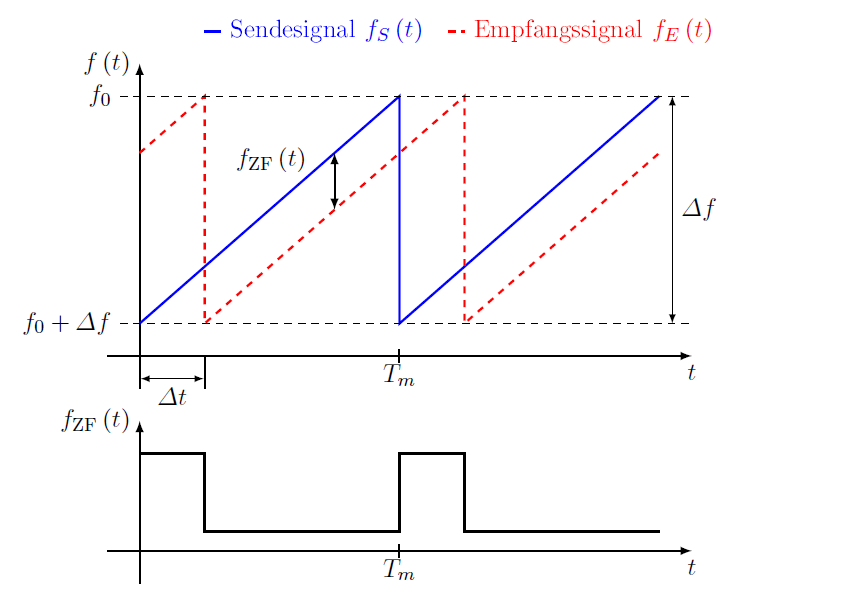
\includegraphics[scale=0.7]{gfx/RadarPHuegler.png}
  \caption{Frequenzverlauf Sende-,  Empfangs-und Zwischenfrequenzsignal\cite[S.6]{Huegler}\cite[S.78]{HuderRadar}}
  \label{fig:FMCW_Frequenz}
\end{figure}
Dabei sind in Abbildung\ref{fig:FMCW_Frequenz} der Frequenzhub $\Delta f$, die Modulationsperiode $T_{m}$ sowie der Frequenzoffset $f_{0}$ dargestellt. Der Frequenzverlauf ist hier als sägezahnförmig angenommen. Andere Formen, beispielsweise sinuförmig oder linear, sind ebenfalls möglich. Zusätzlich wird auf die erste Modulationsperiode beschränkt. Für weitere Perioden gilt das Vorgehen analog.\\
Das Empfangssignal $s_{e}(t)$ wird um den Laufzeitunterschied $\Delta t$ mit
\begin{align}
\Delta t = \frac{2R}{c_{0}}
\end{align}
verschoben. Dabei ist R der Radar-Ziel Abstand. Dadurch ergibt sich für die Empfangsfrequenz $f_{e}(t)$ 
\begin{align}
f_{e}(t) = f_{0} + \frac{\Delta f}{T_{m}}\cdot \left( t-\Delta t \right).
\end{align}
Ist zudem der in Abbildung \ref{fig:FMCWRadar} dargestellte Tiefpass darauf ausgelegt, die Summenfrequenz $f_{s} + f_{e}$ nicht passieren zu lassen, ergibt sich analog zu \cite[S.43,S.44]{HuderRadar} für die Zwischenfrequenz
\begin{align}
f_{ZF}(t) = \vert f_{s}(t)- f{e}(t) \vert = \frac{\Delta f}{T_{m}}\cdot \Delta T.
\end{align}
Damit ist die Zwischenfrequenzspannung $u_{ZF}(t)$ 
\begin{align}
u_{ZF}(t) = u_{ZF} \cdot  \cos\left( 2\pi \frac{\Delta f \Delta t}{T_{m}} \cdot t + \varphi_{s} \right) .
\end{align}
Daraus ergibt sich nach\cite[S.80]{HuderRadar} die Zielentfernung $R$ zu
\begin{equation}
R = \frac{c_{0}T_{m}}{2\Delta f}\cdot f_{ZF}.
\end{equation}
Um $R$ zu bestimmen muss die Zwischenfrequenz gemessen werden. Dafür wird das Zwischenfrequenzsignal verarbeitet und anschließend digitalisiert. Das Spektrum des Digitalsignals kann mit einer FFT\footnote{\textbf{F}ast \textbf{F}ourier \textbf{T}ransformation, eine schnelle Fourier Transformation} berechnet werden. Daraus ergibt sich ein diskretes Spektrum, in dem die Zwischenfrequenz erkennbar ist. Falls mehrere Ziele detektiert werden, lassen sich ebenso mehr Zwischenfrequenzen erkennen.
\section{Rauschen}
Rauschen ist der Sammelbegriff für verschiedene Prozesse die eine eindeutige Signalerkennung erschweren. Das Verhältnis von Signal zu Rauschen ist das $\left( \frac{S}{N}\right)$ mit
\begin{align}
\left( \frac{S}{N}\right) =\frac{Signal}{Rauschen} =  \frac{P_{Signal}}{P_{Rauschen}}.
\end{align}
Das $\left( \frac{S}{N}\right)$ wird ebenfalls als SNR\footnote{\textbf{S}ignal to \textbf{N}oise \textbf{R}atio} bezeichnet. Dabei benötigen viele Systemkomponenten, zum Beispiel ein Empfänger, ein minimales SNR um überhaupt ein Signal rekonstruieren zu können. Das SNR wird meist in dB angegeben.
\section{Link-Budget}
\section{Leitungstheorie}
\subsection{Mikrostreifenleitung}
Eine Mikrostreifenleitung besteht aus einer leitenden Metallschicht, die Leiterbahn, auf den Oberseite eines Substrats. Unter diesem Substrat befindet sich ebenfalls eine leitende Metallschicht, die Massefläche\footnote{Auch Ground-Plane, die Bezugsfläche für das Potenzial}. Dabei sind die \textbf{Substrat-Höhe} $h$, die \textbf{Metallbreite} $W$, die \textbf{Metallhöhe} $d$ sowie die \textbf{Dielektrizität} des Substrats die charakteristischen Größen der Mikrostreifenleitung. Entscheidend\cite{TransmissionLineDesignHandbook} für die Verwendung ist ein Verständnis für die Wellenausbreitung auf der Mikrostreifenleitung. In blablabla ist diese dargestellt. Demnach muss für verschiedene Frequenzen von Wellen die Geometrie der Mikrostreifenleitung angepasst werden. Da sich die elektromagnetische Welle überwiegend innerhalb des Substrats befindet, ist die effektive \textbf{Permittivitätskonstante} $\epsilon_{r,eff}$ eine Möglichkeit die Feldverteilung mathematisch einfach darzustellen. Dabei ist in BLABLABLALBALB dargestellt, wie sich die ursprüngliche Geometrie der Mikrostreifenleitung mit Hilfe von $\epsilon_{r,eff}$ und der \textbf{effektiven Leiterbahnbreite} $W_{eff}$ verändern lässt. Für $\epsilon_{r,eff}$ gilt dabei 
\begin{align}
\epsilon_{r,eff} = \frac{\left( \epsilon_{r}+1 \right)}{2} + \frac{\left( \epsilon_{r}-1 \right)}{2} \cdot \left( 1 + \frac{10h}{W}\right)^{-\frac{1}{2}}.
\end{align}




\subsection{Differentielle Signalübertragung}
Eine differentielle Leitung besteht aus zwei Leiterbahnen. Auf jeder Leiterbahn ist ein Signal, welche zueinander komplementär sind, also $180^\circ $  Phasenverschiebung zueinander haben. Verglichen mit herkömmlichen Leitungen haben differentielle Leitungen einige Vorteile 
\begin{description}
\item Unterschiede im Referenzlevel\footnote{Masse oder GND(engl. für Ground)} zwischen Systemkomponenten haben kaum Einfluss auf Logiklevel.
\item Dämpfung auf einer Leiterbahn ist kompensierbar. Nach \cite{DifferentialSignalLine} lässt sich bis zu 24dB Dämpfung kompensieren.
\item Höhere Datenraten sind möglich. Dabei ist nach \cite{DifferentialSignalLine} bis zu  eine Datenrate von 10Gb/S möglich.
\end{description}
wobei stets mehr Leitungen nötig sind, um die gleiche Anzahl Signale zu führen, wenn pro Signal je eine Leitung verwendet wird. 
\begin{figure}[tbp]
  \centering
  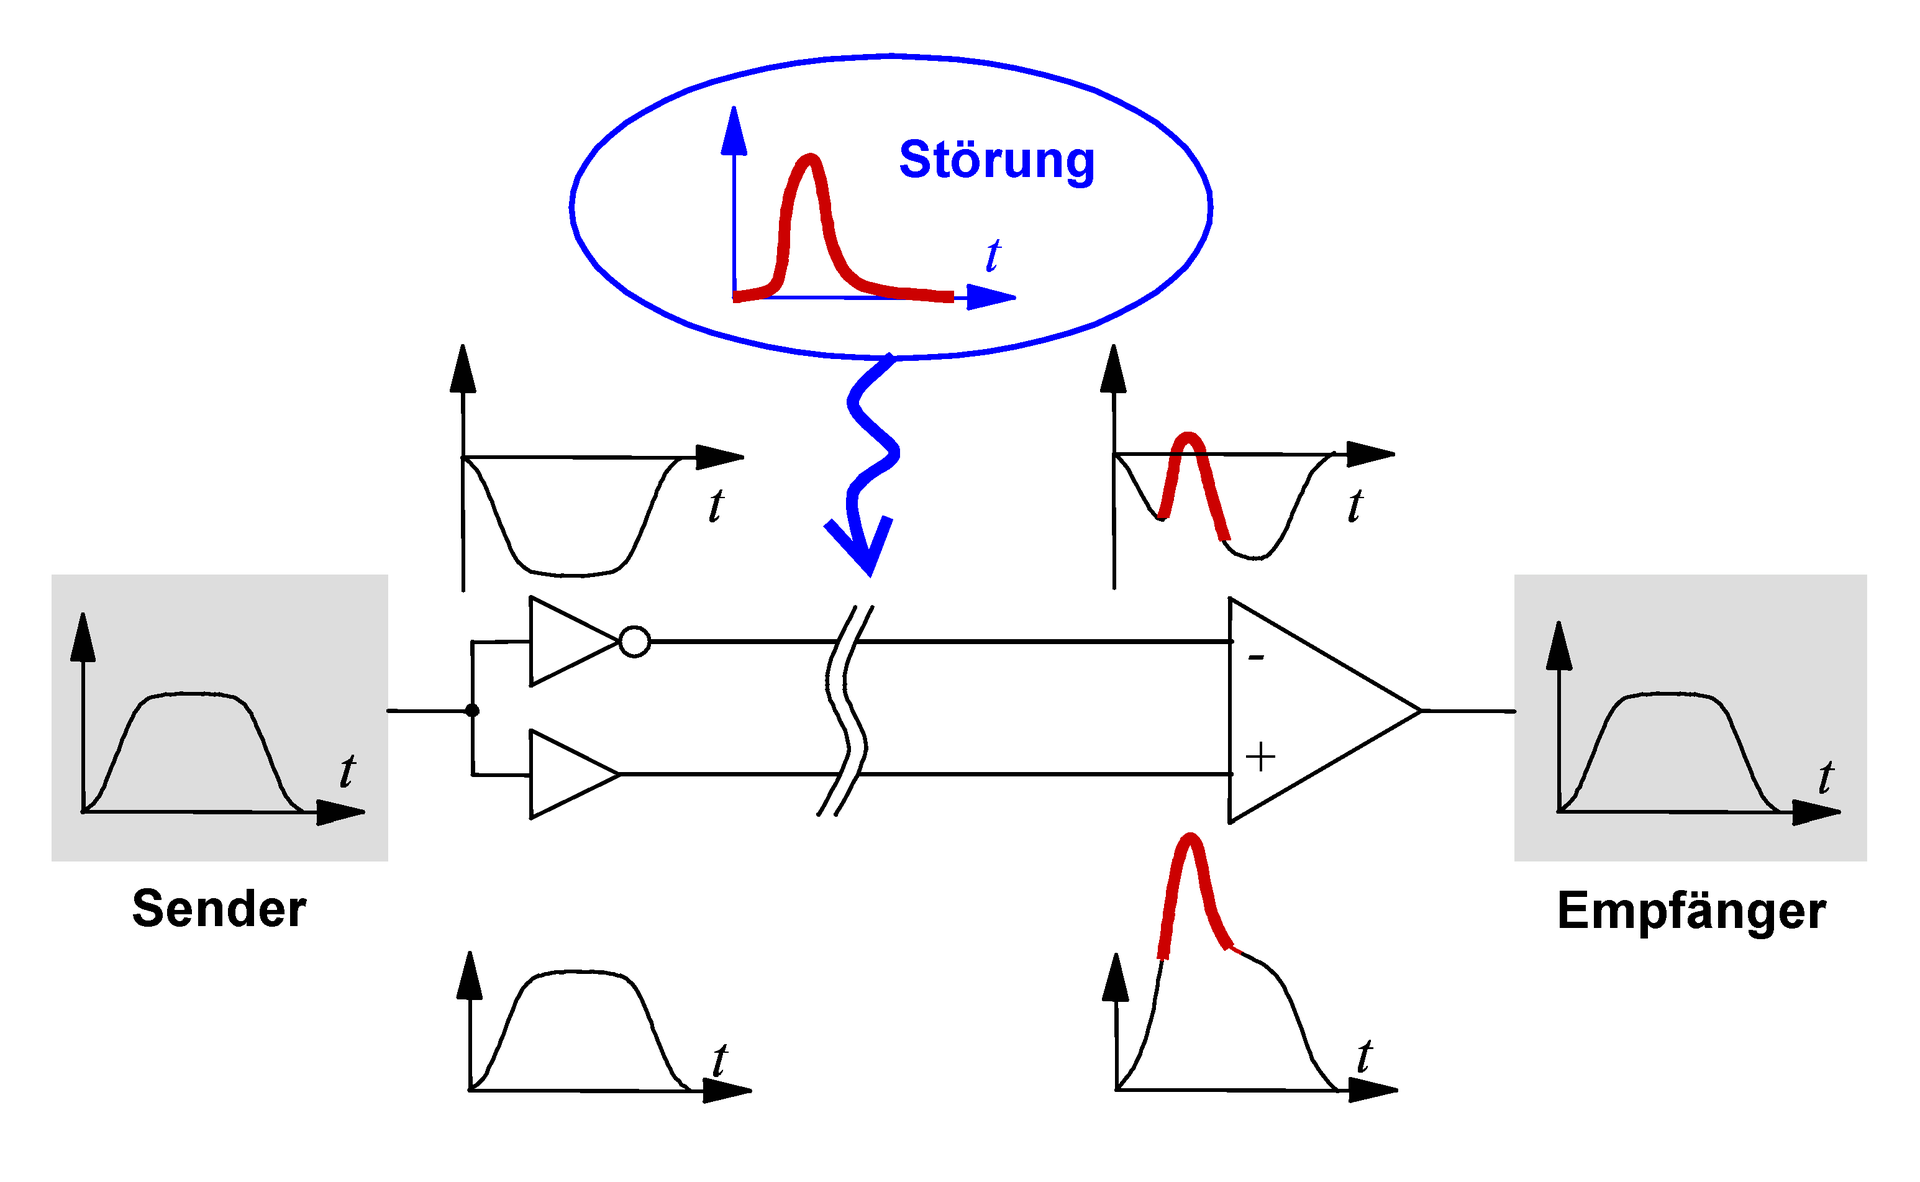
\includegraphics[scale=1.5]{gfx/DiffSignalUebertragung.png}
  \caption{Einfluss einer Störung auf Differentielle Signalübertragung\cite{DiffSig}}
  \label{fig:DiffSig}
\end{figure}
In \ref{fig:DiffSig} ist eine differentielle Leitung dargestellt. Auf beide Signale wirkt dabei die gleiche Störung. Ist auf \ref{fig:DiffSig} die invertierte Leitung $s_{1}$ mit dem dazugehörigen Signal $-s(t)$ sowie die nicht invertierende Leitung $s_{2}$ mit $s(t)$ jeweils die Störung $e(t)$ addiert, ergibt sich durch die Differenz der am Operationsverstärker anliegenden Signale $f$ und $g$ mit 
\begin{align}
f(t) &= -s(t) + e(t) \\
g(t) &=  s(t) + e(t)
\end{align}
als Ausgang $s_{Res}(t)$ von
\begin{align}
s_{Res}(t) = g(t) - f(t)= 2\cdot s(t).
\end{align}
Dabei wird das SNR um 6dB verbessert. Die Längen der jeweiligen Leitungen müssen gleich lang sein. Andernfalls ergibt sich ein Phasenunterschied der eine eindeutige Filterung verhindert. Je nach Frequenz des Signals verhindern bereits kleine Abweichungen die eindeutige Rekonstruktion des ursprünglichen Signals. Diese Abweichungen lassen sich leicht mit \ref{eq:fzulambda} berechnen. Ist die Toleranz der Leitungslänge etwa \SI{1}{\percent} so ist der zulässige \textbf{Leitungslängenunterschied}$\Delta l_{max}$ bei einer Frequenz von \SI{10}{\mega\hertz} $\Delta l_{max} = $ \SI{30}{\centi\meter}, bei einer Frequenz von \SI{2.4}{\giga\hertz} allerdings $\Delta l_{max} =$ \SI{1.25}{\milli\meter}. Der  Leitungslängenunterschied innerhalb einer Toleranz nimmt mit zunehmender Frequenz ab. Je nach Anwendung kann auch ein Bauteil-Takt die Toleranz vorgeben. Zusätzlich muss um eine Störung nur symmetrisch auf beide Leitungen zu erhalten der Leitungsabstand zueinander gering und konstant sein. Je nach Leitungsart ist dies allerdings auf Grund von Feldverteilungen nicht immer möglich.
\subsection{Differentielle Leitungen in Mikrostreifentechnik}
Eine differentielle Mikrostreifenleitung ist in BLABLABLA dargestellt. Für diese ist die \textbf{differenzielle Impedanz} $Z_{Diff}$ nach REFERENZ
\begin{align}
Z_{Diff} = 2\cdot Z_{0} \left(1-0.48\exp^{\left(\frac{-0.96s}{h}\right)}\right)
\end{align} 
gegeben. Dabei ist $s$ der Abstand zwischen beiden Einzelleitungen.

\section{Signalkonditionierung}\label{SignalkonditionierungKapitel}
Signalkonditionierung beschreibt die Bearbeitung eines analogen Signals vor der Weiterverarbeitung in der nächsten, oft letzten, Systemstufe. Dabei ist die letzte Stufe häufig ein ADC\footnote{\textbf{A}nalog-to-\textbf{D}igital-\textbf{C}onverter}. Das analoge Signal wird dabei durch Verstärker, Filter und Konverter manipuliert. Dadurch wird ein besseres SNR erreicht oder die komplette Reichweite eines ADC ausgenutzt, letzteres ist dabei besonders wichtig, da dadurch eine höhere, genauere Auflösung in der digitalen Weiterverarbeitung  erzielt wird. In Abbildung \ref{fig:SigCond} ist eine solche Signalkonditionierung dargestellt. Dabei liegt am Verstärker ein analoges Signal an, dieses wird verstärkt und eventuelles hochfrequentes Rauschen am Tiefpass herausgefiltert. Dann wird das Signal von Analog in Digital umgewandelt. \\
In der Signalkonditionierung wird stets die Kettenrauschzahl beachtet. Durch eine entsprechende Anordnung der Komponenten in Kombination mit differentiellen Leitungen lassen sich so viele Störungen oder Rauschen sehr gut unterdrücken oder herausfiltern. 
\begin{figure}[tbp]
  \centering
  \tikzset{
	block/.style    	= 	{draw, fill=white, thick, rectangle, minimum height = 0.98cm, minimum width = 0.98cm, node distance=2.5cm, line width=1.5pt},
	%
	% Standard circular block
	circleblock/.style	= 	{draw, fill=white, thick, circle, minimum width = 0.98cm,  line width=1.5pt, node distance=2.5cm},
	%
	% Label for circuitikz nodes, as they're reference is in the middle and not on the outer edge of the node....
	circuitikzlabel/.style	=	{label={[label, label distance=0.5cm]#1}},
	%
	%
	%
	% VCO/Oscillator 
	myVCO/.style			= 	{circleblock, path picture={%
		\draw[line width=0.75pt] 	($(path picture bounding box.west)+(0.09cm,0)$) sin ($(path picture bounding box.center)-(0.2cm,-0.2cm)$) cos  (path picture bounding box.center) sin ($(path picture bounding box.center)-(-0.2cm,0.2cm)$) cos ($(path picture bounding box.east)-(0.09cm,0)$);
		}
	},
	% Amplifier, as circuitikz does only provite amplifiers as 2-ports/bipoles
	myAMP/.style		= 	{block, node distance=2.5cm, path picture={%
		\draw[fill=white, line width=0.75pt] ($(path picture bounding box.center)+(0.7em,0)$) -- ($(path picture bounding box.center)-(0.7em,-0.7em)$) -- ($(path picture bounding box.center)-(0.7em,0.7em)$)  -- cycle;
		}
	},
	% Same for ADC
	myADC/.style 	=	{block, path picture={%
		\draw[line width=0.75pt] 	(path picture bounding box.south west) -- (path picture bounding box.north east);
		\node[] at ($(path picture bounding box.center)+(-.5em,.5em)$) () {D};
		\node[] at ($(path picture bounding box.center)+(.5em,-.5em)$) () {A};
		} 
	},
	% Same for filters
	myLP/.style	=	{block, path picture={%
		%Sine-Waves
		\draw[line width=.75pt] 	($(path picture bounding box.west)+(0.3em,0)$) sin ($(path picture bounding box.center)-(0.50em,-0.3em)$) cos  (path picture bounding box.center) sin ($(path picture bounding box.center)-(-0.50em,0.3em)$) cos ($(path picture bounding box.east)-(0.3em,0)$);
		\draw[line width=0.75pt] 	($(path picture bounding box.west)+(0.3em,-0.65em)$) sin ($(path picture bounding box.center)-(0.50em,0.35em)$) cos  ( $(path picture bounding box.center)-(0,0.65em)$) sin ($(path picture bounding box.center)-(-0.50em,0.95em)$) cos ($(path picture bounding box.east)-(0.3em,0.65em)$);
		\draw[line width=0.75pt] 	($(path picture bounding box.west)+(0.3em,0.65em)$) sin ($(path picture bounding box.center)-(0.50em,-0.95em)$) cos  ( $(path picture bounding box.center)+(0,0.65em)$) sin ($(path picture bounding box.center)-(-0.50em,-0.35em)$) cos ($(path picture bounding box.east)-(0.3em,-0.65em)$);
		% Cancelation
		\draw[line width=0.75pt] 	($(path picture bounding box.center)-(0.2em,0.2em)$) -- (path picture bounding box.center) -- ($(path picture bounding box.center)+(0.2em,0.2em)$) ;
		\draw[line width=0.75pt] 	($(path picture bounding box.center)-(0.2em,-0.45em)$) -- ($(path picture bounding box.center)+(0,0.65em)$) -- ($(path picture bounding box.center)+(0.2em,0.85em)$) ;
		}
	},
}
\begin{tikzpicture}[line width=0.7pt,>=latex,node distance=2.5cm]

	\draw (0,0)
		node[myVCO, label={below:Analoges Signal}] (oszi) {}
		node[myAMP, right of = oszi, label={below:Verstärker}] (AMP) {}
		node[myLP, right of = AMP, label={below:Tiefpass}] (LP) {}
		node[myADC, right of = LP ,rotate = 180, label={ADC}] (ADC){}		
		;
		\draw[->] (oszi) -- (AMP);
		\draw[->] (AMP) -- (LP);
		\draw[->] (LP) -- (ADC);

\end{tikzpicture}

  \caption{Einfache Signalkonditionierung}
  \label{fig:SigCond}
\end{figure}
\section{Verstärkergrundlagen}
Ein Verstärker bezeichnet eine Systemkomponente, welche ein  analoges Eingangsignal, in Form von Strom, Spannung oder Leistung, in ein analoges Ausgangssignal nicht zwangsläufig gleicher Art überführt und dieses aktiv verstärkt. Dabei ist die wichtigste Kenngröße die Verstärkung oder auch der Gain. Dabei wird der Gain stets über 
\begin{center}
Ausgangssignal $ = $ Eingangssignal $ \cdot $ Gain
\end{center}
beschrieben. Häufig wird Gain $G$ in dB angegeben, dabei gilt
\begin{equation}
\frac{G}{\text{dB}} = \text{B} \cdot \log \left( \frac{G}{\text{lin}} \right).
\end{equation}
Dabei ist 
\begin{equation}
\text{B} = \begin{cases} 20 \text{ , falls Signal Spannung oder Storm} \\ 10 \text{ , falls Signal Leistung} \end{cases}.
\end{equation}
Dabei unterscheiden sich verschiedene Verstärkertypen. Einige sind folgend aufgezählt.

\begin{description}
\item Stormverstärker \\
	  Eingangsstrom in Ausgangsstorm
\item Spannungsverstärker    		\\
	  Eingangsspannung in Ausgangsspannung
\item Transkonduktanzverstärker   \\
	  (Eingangsspannung  in Ausgangsstrom
\item Transimpedanzverstärker  	\\
Eingangsstrom  in Ausgangsspannung
\end{description}
Zusätzlich lassen sich Verstärker bezüglich ihrer Funktion oder Verwendung  charakterisieren. Es wird sich weiterhin auf Operationsverstärker beschränkt. In Abbildung \ref{fig:OpAmp} ist ein solcher dargestellt. Operationsverstärker haben einen differentiellen Eingang und verstärken Spannungen, sind also ein Spannungsverstärker. Dabei soll die Differenz der Eingänge $U_{in,p}$ und $U_{in,n}$ die Ausgangsspannung $U_{aus}$ bestimmen. Also gilt
\begin{equation}
U_{aus} = G \cdot \left( U_{in,p} - U_{in,n}\right).
\end{equation} Dabei hat der Operationsverstärker meist nur einen Ausgang. Differentielle Ausgänge werden im Anschluss durch invertieren eines Eingangs erzeugt. Invertiert wird durch einen Operationsverstärker mit $G = -1$ sowie dem negativem Input auf dem Bezugspotenzial.\\ 
Ein Operationsverstärker benötigt eine eigene Versorgungsspannung $V_{S}$. Diese gibt die maximale Ausgangsspannung an. Die Eingangsimpedanz des Operationsverstärkers sollte hoch sein. In idealen Operationsverstärkern wird sie als $\text{Z}_{in} = \inf$ angenommen. Dagegen ist die Ausgangsimpedanz möglichst klein, in idealen Operationsverstärkern wird diese als $\text{Z}_{aus} = 0$ angenommen. Also sind beide einfließenden Ströme $I_n = I_p = 0$.
\begin{figure}[tbp]
  \centering
  \begin{tikzpicture}[scale=2]
        \draw
        (0, 0) node[op amp,scale = 2] (opamp) {}
		(opamp.+) node[left] {$U_{in,n}$}
		(opamp.-) node[left] {$U_{in,p}$}
		(opamp.out) node[right] {$U_{aus}$}
		(opamp.up) --++(0,0.5) node[vcc]{$V_{S}$}
		(opamp.down) --++(0,-0.5) node[vee]{$-V_{S}$
}		     
        ;
\end{tikzpicture}

  \caption{Symbol eines Operationsverstärker}
  \label{fig:OpAmp}
\end{figure}
\subsection{Systemparameter von Operationsverstärkern}
Reale Operationsverstärker haben einige nicht ideale Effekte. Um diese zu beschreiben, werden Operationsverstärker mit einigen Parametern beschrieben
\begin{description}
\item Endlicher Gain \\
Dabei gilt es zwischen Open-Loop-Gain und Closed-Loop-Gain zu unterscheiden. Der Open-Loop-Gain bezeichnet die mögliche Verstärkung der Operationsverstärkers, wenn keine Rückführung auf die Eingänge vorhanden ist. Der Open-Loop-Gain eines idealen Operationsverstärkers ist $\inf$. Auch in realen Operationsverstärkern kann dieser Wert sehr groß werden. Der Closed-Loop-Gain wird durch die Beschaltung der Rückführung bestimmt sowie die Verhältnisse der dortigen Komponenten, meist Widerstände, definiert.
\item Eingangsimpedanz \\
Die differentielle Eingangsimpedanz gibt die Impedanz zwischen positiven und  negativen Eingang des Operationsverstärkers an. Die Gleichtakt Eingangsimpedanz, auch Common-Mode Impedanz, beschreibt die jeweilige Impedanz bezogen auf das Massepotenzial.
\item Gleichtaktunterdrückung \\
Gleichtaktunterdrückung CMR\footnote{ \textbf{C}ommon \textbf{M}ode \textbf{R}ejection} beschreibt die Änderung von $U_{aus}$ wenn sich beide Eingänge um den gleichen Wert ändern. Ein wesentliche Maß für die Qualität eines Operationsverstärkers ist die Gleichtaktunterdrückung. Dabei soll diese möglichst groß, idealerweise unendlich groß sein. Entsprechend ist die Gleichtaktverstärkung idealerweise null. 
\item Slew Rate und Bandbreite \\
Da ein Operationsverstärker stets seinen Eingängen folgt, ist dies nur bis zu einer maximalen Geschwindigkeit möglich. Diese Geschwindigkeit ist die Slew Rate. Ist die Änderung schneller als der Operationsverstärker, wird nicht mehr der volle Gain erreicht. Sobald der Gain um \SI{3}{dB} kleiner ist als vorgesehen, ist die Bandbreite überschritten.
\item Ausgangsrauschen\\
Da Operationsverstärker aktive Bauelemente sind, erzeugen diese stets auch ein eigenes Rauschen welches dem bisherigen Rauschpegel hinzugefügt wird. Ein wesentliches Qualitätsmerkmal eines Operationsverstärkers ist dabei das Ausgangsrauschen. Ein idealer Operationsverstärker hat dabei kein Ausgangsrauschen. In der Realität hängt es allerdings von Lastwiderstand sowie Gain ab. 
\item Interception Point 3 \\
Interception Points modellieren die in der Realität vorhandenen Nichtlinearitäten von Operationsverstärkern mit Hilfe von Polynomen niedriger Ordnung, beispielsweise einer Taylorentwicklung. Der Interception Point 3 bezeichnet demnach den Einfluss der nichtlinearen Terme dritter Ordnung. Dabei ist der Interception Point 3 keine physikalische Größe. Effektiv beschreibt der Interception Point 3 die dynamische Reichweite bzw. die Grenze davon. 
\end{description}

\section{Filtergrundlagen}

\section{Phasenregelschleife}
Eine Phasenregelschleife, auch PLL\footnote{ \textbf{P}hase \textbf{L}ocked \textbf{L}oop}, ist ein geschlossener Regelkreis der eine stabile Ausgangsfrequenz mit Hilfe einer Referenzfrequenz herstellt. Dabei wird eine PLL insbesondere bei der Taktgebung in Systemen verwendet. Bild \ref{fig:PLL_Blockerino} zeigt eine solche PLL als Blockschaltbild und wird weiterhin näher erläutert. Dabei wird ein Referenzfrequenzgeber, zwei Frequenzteiler, ein Phasendetektor, ein Schleifenfilter und ein Voltage Controlled Oscillator benötigt.
\begin{figure}[tbp]
  \centering
  \tikzset{%
	% Self defined bulding blocks. 
	% Nevertheless circutikz has implemented filters, couplers and other components since version 0.4, they are mostly implemented as bipoles.
	% The usage of bipoles: \draw (start) to[lowpass/amp/adc,....] (end).
	% The problem is, that if one wants to use arrows, the arrows in bipoles can not be sat manual (fixed in circuitikz source) AND THEY ARE NOT CONSISTENT
	% Also it's quite a mess, which component is a monopole, simple block, bipol, quad/triple etc
	% Following are a few examples on how to define your own blocks. 
	%
	% % % % % % % % % % % % % % % % % % % % % % % % % % % % % % % % % % % % % % % % % % % % % % % % % % % % % % % % % % % % % % % % % % % % %
	% % % % % % % % % % % % % % % % % % % % % % % % % % % % % % % % % % % % % % % % % % % % % % % % % % % % % % % % % % % % % % % % % % % % %
	% % % % % % % % % % % % % % % % % % % % % % % % % % % % % % % % % % % % % % % % % % % % % % % % % % % % % % % % % % % % % % % % % % % % %
	% % % % % % % % % % % % % % % % % % % % % % % % % % % % % % % % % % % % % % % % % % % % % % % % % % % % % % % % % % % % % % % % % % % % %
	%
	% Standard block definition, the width and height is adopted from the circutizk source code, so don't mind the strange values. Also the linewidth is set according to the circutrikz source code.
	block/.style    	= 	{draw, fill=white, thick, rectangle, minimum height = 0.98cm, minimum width = 0.98cm, node distance=2.5cm, line width=1.5pt},
	%
	% Standard circular block
	circleblock/.style	= 	{draw, fill=white, thick, circle, minimum width = 0.98cm,  line width=1.5pt, node distance=2.5cm},
	%
	% Label for circuitikz nodes, as they're reference is in the middle and not on the outer edge of the node....
	circuitikzlabel/.style	=	{label={[label, label distance=0.5cm]#1}},
	%
	%
	%
	% VCO/Oscillator 
	myVCO/.style			= 	{circleblock, path picture={%
		\draw[line width=0.75pt] 	($(path picture bounding box.west)+(0.09cm,0)$) sin ($(path picture bounding box.center)-(0.2cm,-0.2cm)$) cos  (path picture bounding box.center) sin ($(path picture bounding box.center)-(-0.2cm,0.2cm)$) cos ($(path picture bounding box.east)-(0.09cm,0)$);
		}
	},
	% Amplifier, as circuitikz does only provite amplifiers as 2-ports/bipoles
	myAMP/.style		= 	{block, node distance=2.5cm, path picture={%
		\draw[fill=white, line width=0.75pt] ($(path picture bounding box.center)+(0.7em,0)$) -- ($(path picture bounding box.center)-(0.7em,-0.7em)$) -- ($(path picture bounding box.center)-(0.7em,0.7em)$)  -- cycle;
		}
	},
	% Block	
	myBlock/.style    	= 	{draw, fill=white, thick, rectangle, minimum height = 0.98cm, minimum width = 0.98cm, node distance=2.5cm, line width=1.5pt},
	myBigBlock/.style    	= 	{draw, fill=white, thick, rectangle, minimum height = 0.98cm, minimum width = 2.94cm, node distance=2.5cm, line width=1.5pt},	
	% Same for ADC
	myADC/.style 	=	{block, path picture={%
		\draw[line width=0.75pt] 	(path picture bounding box.south west) -- (path picture bounding box.north east);
		\node[] at ($(path picture bounding box.center)+(-.5em,.5em)$) () {D};
		\node[] at ($(path picture bounding box.center)+(.5em,-.5em)$) () {A};
		} 
	},
	% Same for filters
	myLP/.style	=	{block, path picture={%
		%Sine-Waves
		\draw[line width=.75pt] 	($(path picture bounding box.west)+(0.3em,0)$) sin ($(path picture bounding box.center)-(0.50em,-0.3em)$) cos  (path picture bounding box.center) sin ($(path picture bounding box.center)-(-0.50em,0.3em)$) cos ($(path picture bounding box.east)-(0.3em,0)$);
		\draw[line width=0.75pt] 	($(path picture bounding box.west)+(0.3em,-0.65em)$) sin ($(path picture bounding box.center)-(0.50em,0.35em)$) cos  ( $(path picture bounding box.center)-(0,0.65em)$) sin ($(path picture bounding box.center)-(-0.50em,0.95em)$) cos ($(path picture bounding box.east)-(0.3em,0.65em)$);
		\draw[line width=0.75pt] 	($(path picture bounding box.west)+(0.3em,0.65em)$) sin ($(path picture bounding box.center)-(0.50em,-0.95em)$) cos  ( $(path picture bounding box.center)+(0,0.65em)$) sin ($(path picture bounding box.center)-(-0.50em,-0.35em)$) cos ($(path picture bounding box.east)-(0.3em,-0.65em)$);
		% Cancelation
		\draw[line width=0.75pt] 	($(path picture bounding box.center)-(0.2em,0.2em)$) -- (path picture bounding box.center) -- ($(path picture bounding box.center)+(0.2em,0.2em)$) ;
		\draw[line width=0.75pt] 	($(path picture bounding box.center)-(0.2em,-0.45em)$) -- ($(path picture bounding box.center)+(0,0.65em)$) -- ($(path picture bounding box.center)+(0.2em,0.85em)$) ;
		}
	},
}
\begin{tikzpicture}[line width=0.7pt,>=latex,node distance=2.5cm]
	% First: All building blocks are placed relative to the first component
	\draw (0,0)
		node[myVCO, label={above:Referenzquartz}] (Ref) {}
		node[myBlock,right of = Ref,label={above:R-Teiler}](QQW){$\frac{1}{R}$}
		node[myBlock,right of = QQW,label={above:PD/CP}](Odda){$f_{pd}$}
		node[myBlock,right of = Odda,label={above:Schleifenfilter}](LFF){$Z(s)$}
		node[myBlock,below of = LFF,label={below:N-Teiler}](NNN){$\frac{1}{N}$}
		node[myVCO, right of = LFF,label={above:VCO}] (RRef) {}
		node[right of = RRef](penis){}
		
		;
	\draw[->] (Ref) -- node[above]{$f_{ref}$}(QQW);
	\draw[->] (QQW) -- node[above]{$f_{comp}$}(Odda);
	\draw[->] (Odda) -- node[above]{$i_{CP}$}(LFF);
	\draw[->] (LFF) -- node[above]{$u_{VCO,in}$}(RRef);
	\draw[->] (RRef) |- node[right]{$f_{out}$}(NNN);
	\draw[->] (NNN) -| node[left]{$f_{n}$}(Odda);
	\draw[->] (RRef) -- node[above]{$f_{out}$}(penis);
	% Connect everything together


\end{tikzpicture}

  \caption{Blockschaltbild Phasenregelkreis nach \cite[S.9]{PLL_Perf}}
  \label{fig:PLL_Blockerino}
\end{figure}
Grundlage bei einer PLL ist stets eine stabile Referenz-Frequenz $f_{ref}$. Häufig wird diese durch einen Quarzoszillator erhalten. Der R-Teiler teilt die Frequenz in eine niedrigere, die Kompensationsfrequenz $f_{comp}$ mit 
\begin{align}
f_{comp} = \frac{f_{ref}}{R}.
\end{align} 
Diese Frequenz ist einer der Eingänge des Phasendetektors, PD. Der Phasendetektor gibt eine Spannung die dem Phasenfehler zwischen seinen beiden Eingängen, $f_{comp}$ und $f_{n}$, entspricht .  Dabei ist $f_{n}$ die durch den N-Teiler rückgeführte Ausgangsfrequenz. Die Charge Pump CP wandelt diese Spannung dabei in einen Strom $i_{CP}$ um. Der Phasendetektor hat dabei noch einen Proportionalität-Faktor $K_{\varphi}$. $K_{\varphi}$ ist dabei die Amplitude die die Charge-Pump verarbeiten kann. Wird $i_{CP}$ mit der Impedanz des Schleifenfilters $Z(s)$ multipliziert, was dem Ohmschen Gesetz entspricht, ergibt sich für den Voltage Controlled Oscillator VCO der Eingang 
\begin{align}
u_{VCO,in} = i_{CP}\cdot Z(s).
\end{align} 
Der Schleifenfilter ist dabei ein Tiefpass um lediglich die gewünschte Spannung an den VCO anzulegen. Der VCO ist ein Spannung-zu Frequenzwandler. Dabei hat der VCO einen Proportionalität-Faktor $K_{VCO}$. Demnach gilt für $f_{aus}$
\begin{align}
f_{aus} = \frac{R}{N} \cdot f_{Ref}.
\end{align} 
Durch ein hohes $R$ sowie ein kleines $N$ lassen sich somit Frequenzen in nahezu beliebiger Höhe erreichen, welches durch Referenzquarze nicht möglich ist, da diese häufig nur bis \SI{200}{\mega\hertz} verfügbar sind. Zusätzlich lässt sich dadurch eine niedrige Referenzfrequenz verwenden. Diese sind stabil und demnach ergibt sich geringeres Phasenrauschen am VCO.\\
Häufig wird der Begriff PLL für das gesamte Bild \ref{fig:PLL_Blockerino} verwendet, mit Ausnahme von Referenzquarz und VCO. Diese sind nach \cite[S.10]{PLL_Perf} schwer auf einen PLL Chip zu integrieren.\\
Entscheidende Parameter für die Leistung der PLL sind das Phasenrauschen und die Einrastzeit. Wesentlich für das Phasenrauschen ist dabei der N-Teiler Wert. Je kleiner dieser Wert desto kleiner das Phasenrauschen \cite[S.10]{PLL_Perf} . Die Einrastzeit ist die Dauer die die PLL für die Frequenzänderung benötigt, wenn der Wert des N-Teilers geändert wird.
\section{PCB Designprozess IF-Board}
Zunächst wurde ein schematisches Design der Signalkette erzeugt. In diesen wird bereits die Form der Spannungsversorgung sowie die Form der zusätzlichen Bauteile wie Widerstände oder Kapazitäten festgelegt. Dieses " Schematic" wird im Anschluss in eine " Netlist" exportiert. Diese beschreibt welches Bauteil mit welchen anderen Bauteilen verbunden ist und gibt diesen Verbindungen, den " Nets" je einen Namen. Diese Netlist wird in eine PCB-Design Umgebung importiert. In dieser wird das eigentliche Platzieren der Bauteile vorgenommen. \\
Die verwendete Software ist eine Cadence Orcad bzw. eine Cadence Allegro Kombination. In Orcad wird das Schematic sowie die Netlist erstellt,in Allegro dann das eigentliche PCB-Design. Zusätzlich wurde ein Pad-Design Programm verwendet um gegebenenfalls noch nicht vorhandene Bauteile für den Deisgn-Prozess zu entwerfen. Dabei wird nicht das Bauteil neu erfunden, sondern die Verbindung einer Komponente auf das PCB in Form von SMD-Pads\footnote{\textbf{S}urface \textbf{M}ounted \textbf{D}evice}. \\

\subsection{Lagenaufbau und Substratauswahl}
Für die Zwischenfrequenzplatine wird FR4 als Substrat Material verwendet. FR4 ist ein gebräuchliches Substrat Material aus Epoxydharz-Glasfaser-Gewebe in der PCB-Herstellung. Die Eigenschaften von FR4 sind in Tabelle \ref{tab:FR4} dargestellt, wobei insbesondere der niedrige Preis und die einfache Verarbeitung, d.h. das Substrat ist fest und demnach nicht leicht verformbar, im Vergleich zu anderen Substraten von Vorteil ist. Die gebräuchliche Substrat-Dicke liegt zwischen  $\SI{0.254}{m\meter}$  und $\SI{1.5}{m\meter}$ . Auf das Substrat wird Kupfer mit einer Dicke von $\SI{18}{u\meter}$ bis $\SI{35}{u\meter}$ aufgetragen. Zusätzlich sind Vier Lagen vorgesehen um den Signalpfad bestmöglich von potenziellen Störquellen zu isolieren.\\
Zwei der Vier Lagen sind führen Signale, eine auf der Oberseite, eine auf der Unterseite. Die beiden Innenlagen sind eine Power-Plane und eine Ground-Plane, zusammenfassend PGP\footnote{\textbf{P}ower\textbf{G}round\textbf{P}lane} genannt.  PGPs dienen zur Verteilung von Versorgungsspannungen oder einem einheitlichen definierten Bezugspotenzial über das gesamte Board. Zusätzlich sind beide Arten von PGPs wichtig zur Wärmeableitung sowie zur Abschirmung von der oberen bzw. unteren Signalebene. 
\begin{table}[tbp]
  \centering
  \begin{tabular}{lr}
    Parameter                               & Value\\
    \hline
    Substratmaterial        & FR4\\
    Substratdicke                           & \SI{0.8}{m\meter}\\
    Dielektrizitätszahl $\epsilon_{r}$ & 5.0 \\
    Verlustfaktor $\tan \left( \delta \right)$ & 0.02 \\
    Oberflächenwiderstand & $\geq$\SI{10}{\kilo\ohm} \\
    Durchgangswiderstand & $\geq$\SI{10}{\kilo\ohm} \\
  \end{tabular}
  \caption{FR4 Materialparameter}
  \label{tab:FR4}
\end{table}
Die verschiedenen Lagen werden durch Through-Vias hergestellt. Dabei bezeichnen Through-Vias Durchkontaktierungen durch sämtliche Lagen. Dabei wird, falls in einer Lage keine Verbindung erforderlich ist, um das Via herum eine Fläche ausgespart. Dadurch hat das VIA keinen Kontakt mit der entsprechenden Lage. Wichtig sind die bei der Fertigung auftretenden Herstellungstoleranzen. Die Dicke einzelner Lagen kann sich um bis zu \SI{20}{\percent} verändern. Ebenfalls können sich einzelne Lagen zueinander verformen. Dabei sind besonders Innenlagen betroffen. Auch Bohr- oder Ätzungenauigkeiten sind zu berücksichtigen. Dabei sollten stets \SI{20}{\micro\meter} Toleranz bedacht werden. Demnach muss bei der Dimensionierung einer Komponente beachtet werden, dass die Größe um $\pm \SI{20}{\micro\meter}$ variiert. Dies tritt insbesondere bei Abständen von Komponenten zueinander auf. Jeder Abstand sollte demnach mindestens doppelt so groß sein wie die einfache Toleranz.
\subsection{Signalleitung}
Signale oder Spannungen werden auf Kupfer geleitet. Dabei werden Spannungen eher über Ebenen geführt als über Leitungen mit konstante Breite. Dies resultiert aus der umgekehrten Proportionalität der Leitungsbreite zum Leitungswiderstand. Ein geringer Widerstand sorgt dabei für geringe Spannungsverluste auf dem PCB.\\
Signale werden entweder Single-Ended oder Differentiell geführt. Besonders digitale Signale sind dabei Single-Ended. Das eigene Zwischenfrequenzsignal wird auf dem PCB Differentiell geführt und erst mit der letzten Systemkomponente Single-Ended umgewandelt.\\
Die zu erwartende Bandbreite sind bis zu \SI{20}{\mega\hertz}. Bei diesen Frequenzen sind geringe Längenunterschiede in der differentielle Leitung tolerierbar, da bei angenommenen \SI{20}{\mega\hertz} ein Längenunterschied von \SI{8}{c\meter}, der gesamten Länge des PCB, nur ein relativer Fehler von 0.01875 oder von 10.6 Grad Phase auftritt. Da ein Fehler dieser Größenordnung bedeutet, dass eine Leitung über das gesamte PCB führt und die andere nicht existiert, kann der Fehler durch Längenunterschiede als klein genug angenommen werden um nicht weiter berücksichtigt zu werden.\\
Entsprechende Signalleitungen sind stets von Through-Vias umgeben. Diese sorgen für einheitliche Referenzpotenziale um die Leitungen herum. Zusätzlich sind Knicke von mehr als \SI{45}{\degree} zu vermeiden. Bei stärkerem Knick ändert sich abrupt die Impedanz der Leitung und verursacht demnach Reflexionen, die vermieden werden müssen. Theoretisch wären Leiterbahnbögen die beste Wahl, allerdings sind diese in der Herstellung deutlich aufwändiger im Vergleich zu \SI{45}{\degree} Winkeln und bringen dabei keine wesentliche Fortschritte in den betrachteten Frequenzen.\\
\subsection{Komponenten Auswahl}
Über eine Stiftleiste wird das auf die Zwischenfrequenz gemischte Signal auf die Platine gegeben. Dieses Signal ist der Ausgangspunkt für die Komponentenwahl. Ziel ist es, ein für die AD-Wandlung konditioniertes Signal an die SMA-Verbinder zu leiten. Da das Ausgangssignal differentiell vorliegt, ist das Ziel einer Systemkomponente die Umwandlung von differentiell auf Single-Ended. Dies wird der Systembaustein, da die differentielle Übertragung wie bereits in XYZ beschrieben vorteilhaft ist in Bezug auf die Störanfälligkeit. Demnach wird eine differentielle Signalführung möglichst lange aufrechterhalten. Diese Systemkomponente wird als BALUN\footnote{Balanced-Unbalanced} bezeichnet. Ausgewählt wurde der ADA4841-2 von Analog Deviced. Der ADA4841-2 hat eine Bandbreite von \SI{80}{\mega\hertz} und bei kleinen differentiellen Signalamplituden von bis zu \SI{400}{m\volt} von Spitze zu Spitze stets eine Bandbreite von \SI{20}{\mega\hertz}. Generell ist es möglich mehr Gain zu erzeugen, allerdings soll der ADA4841-2 insbesondere den Analog-Digital-Wandler antreiben. Dementsprechend wird der ADA4841-2 als eine Form von Buffer, nicht als Verstärker angesehen. Das entscheidende Kriterium um einen Analog-Digital-Wandler anzutreiben ist das niedrige Ausgangsrauschen. Verstärker erzeugen im Allgemeinen mehr Rauschen als einfache Buffer. Diese Voraussetzung erfüllt der ADA4841-2. \\
Eine weitere zentrale Systemkomponente ist die Kombination Verstärker mit Tiefpass. Für diese Kombination wurde der HMC900 sowie der HMC960 von Analog Devices ausgewählt. Beide sind bereits von Werk aufeinander eingestellt. Dabei ist der HMC960 ein programmierbarer Verstärker mit einstellbarem Gain. Die Bandbreite des HMC960 sind \SI{100}{\mega\hertz}
\begin{table}[tbp]
  \centering
  \begin{tabular}{l c c c c}
    Feature & ADA4937 & HMC960 & HMC900 & ADA4841\\
    \hline
    Gain(dB) & 0-14 & 0-40 & 0/10 & 1-20 \\
    Bandbreite(MHz) & 1900 & 180 & 50 &\\
    Rauschen(nV/$\sqrt{\text{Hz}}$) & 5.8-16.2& 6-125 & 25 &2-40\\
    Rauschen(dB) & 15 & 23-6 &25/17 & \\
    IP3(dBm) & tbd & 32 &30&\\
  \end{tabular}
  \caption{Parameter der Systemkomponenten Zwischenfrequenzplatine}
  \label{tab:IFKomponenten}
\end{table}

\begin{table}[tbp]
  \centering
  \begin{tabular}{l r}
    Parameter & Wert\\
    \hline
	Gain(dB) & 0-40\\
	Bandbreite(MHz) & 180 \\
	Ausgangsrauschen(nV / rtHz) &   9-125 \\
	Noise Figure (dB) & 23-6.1\\
	Ausgangs Interception Point(dBm) 3 & 32-33\\
	Input Common-Mode-Range(V) & 1-4 \\
	
  \end{tabular}
  \caption{HMC960}
  \label{tab:HMC960}
\end{table}